% !TeX root = SketchFace.tex

\section{Deep Network for Sketch-Photo Translation}
\label{sec:network}

\subsection{Edge alignment in baseline Model}

Generating a realistic photo from sketch can be considered as an image translation problem. 
We use the state-of-the-art Pix2PixHd~\cite{} as our baseline. 
% 
 
We use the CelebA-HD dataset~\cite{} which contains \td{xxx face images in WxH}. All the face images are globally aligned according to their eye positions. 
For each photo, we generate sketch samples \td{by xxx method}.
\td{XX for training and xx for testing.}
%
Using this paired sketch-photo dataset, \td{we trained our method and other state-of-the-art approaches for comparison}.

\subsubsection{Global alignment}
While all the face images in the CelebA dataset \cite{} are globally aligned with their eye positions, the learned generator implicitly embeds the global layout. Once the drawn sketches deviate from this implicitly embedded layout, the learned translation model generate awkward results, as Fig.~\ref{fig:global-align-fail} shows. 


\begin{figure}
	\centering
	\vspace{1.0cm}
	\caption{Generated face images from a sketch that does not follow the aligned face layout.}
	\label{fig:global-align-fail}
\end{figure}

\subsubsection{Data augmentation with geometric translation}
A straightforward way is to augment the training set by random geometric transformation of input sketches. 
However, large interval/range of the transform yields un-convergence of the network training. 
We limit the transformation range to $(-\frac{\pi}{10},\frac{\pi}{10})$ rotation, $(-\frac{W}{20},\frac{W}{20})$ translation, and \cxj{scale?} in order to increase the tolerance of the trained model on the distortion and roughness of hand-drawn sketches. 
%
Moreover, as an interactive system, we also simply provide a reference sketch, like ShadowDrawing~\cite{}.
We place an averaged face contour image on the canvas to provide a reference coordinate system for user to draw their strokes. 
Therefore, the drawn sketches under this geometric reference will be located in or close to space of the training sketches.

%%%% \subsubsection{Data augmentation with sketch dilation}
% !TeX root = SketchFace.tex

\subsubsection{Face Sketches and Data Augmentation}
Paired face sketch-photo dataset is required for supervised sketch-to-face generation methods.
Since there exits no large-scale face sketch datasets, the training face sketches used by existing methods are generated from face image dataset, e.g. CelebA-HQ face dataset, using edge detection algorithm such as HED~\cite{HED}.
However, the sketches generated by edge detection algorithm are sometimes incomplete or \td{other problems}. 
\cxj{I would say the edge maps are quite different from handdrawn sketches, not because of the incompleteness.}
\rmv{ Although CSAGAN~\cite{CSAGAM} applied self-attention mechanism to alleviate the incompleteness problem, the others remains. Therefore we use another method to generate clearer and complete sketches from face images.}
The CelebAMask-HQ dataset~\cite{CelebAMask-HQ} provides a face semantic map for each face image in CelebA-HQ dataset. We basically use the boundary map of the semantic map as the sketch of the corresponding face image. Figure~\ref{fig:sketch_data} shows an example of comparison between a sketch generated by edge detector and from semantic boundary.
%
A contour2photo model is trained in Pix2PixHd to generate face images from face contours that contains facial makers only. Hair shapes, or other facial features such as beard, wrinkles, are not supported. 
\cxj{Compare with contour data? With different styles of input sketches, the trained model is not well generalized. }

\paragraph{Stroke Deformation}
A shortcut of sketches generated from semantic boundary (and those generated by edge detector) is the lines of sketches are perfectly aligned to the edges of the corresponding face images. In order to break the edge-alignment and mimic the hand-drawn sketches, we apply a deform to the lines. Specifically, we vectorize the lines of each sketches using AutoTrace algorithm~\cite{AutoTrace}, and add an offset randomly selected from $[-d, d]^2$ to the control points and end points of the vectorized lines, where $d$ is the maximum offset and we set $d=11$ in our experiments.


\begin{figure}
	\centering
	\vspace{1.0cm}
	\caption{Comparison between a sketch generated from edge detection and from semantic boundary.}
	\label{fig:sketch_data}
\end{figure}

\subsubsection{pix2pixHD without instance normalization}
The baseline model, as well as many existing stylization DNNs, uses spatial normalization to extract style statistics, treating them as spatially uniform on the entire image. 
However, the shallow convolution layers typically extract texture or brightness statistics, which are varying dramastically on different local regions of a drand-drawn sketch. For example, there might be a large number strokes around hair regions or mouth regions to describe details. These heavy strokes bring significant difference while instance normalization at each convolution layer normalizes local patch features with a global factor. Therefore, the extracted features for identical eye strokes could be very different. 

We think that strokes mainly describe the shape features, without little texture information. 

%%% \subsubsection{Spatial Attention Pooling}
% !TeX root = SketchFace.tex

\subsubsection{Spatial Attention Pooling}
When the input hand-drawn sketch is not well-drawn, it is a trade-off between the realism of the output face image and the alignment between the input sketch and the output face image.
%
In order to alleviate the edge alignment between the input sketch and the output face image, we should relax the sharp sketch lines with one-pixel width.
\cxj{relax thin strokes to an ambiguity band with various width or uncertainty.}
One of the straightforward ways is to smooth the lines of sketches using image smoothing algorithm. 
Another is to dilate the sketch lines so that the widths of lines are of multiple pixels~\cite{DeepSurgery}.
\cxj{if it is not officially published, it is not necessary to cite it. but if our method performs better, then cite it and show comparison.}
However, the capacity of either the two hand-crafted ways above is limited, \td{because the uniform smoothness and the dilate radius for all positions of the whole sketch violate the unevenness of hand-drawn sketches on depicting different facial parts. }
%
We argue that the balance between the realism of the output face image and the alignment between the input sketch and the output face image differs from one position to another across the face image. Therefore, the smoothness or the dilation radius should be spatial-specific. 

Based on the discussion above, we propose a new module, called spatial attention pooling (SAP), to dilate the input sketch in a spacial-specific way. 
\cxj{I would not use 'dilate' since this simple word does not reveal the underlying discovery.}
%Let $\mathbf{r}=\{r_i | i=1,2,...,N_r\}$ be a set of dilation radius. 
Given an input sketch $S\in \real^{H\times W}$, we first pass it through $N_r$ pooling branches with different kernel sizes of $r_i, i=1,\ldots, N_r$ to get $\{P_{i}| i=1,\ldots,N_r\}$. 
Then we compute the spatial attention map $W\in \real^{N_r\times H\times W} $with $W = Softmax(f(s))$, where $f()$ is implemented with two convolutional layers. \cxj{$f(S)$ to extract low-level features from the input sketch?}
\cxj{It is not clear what is the motivation of computing the SA map $W$. It might be better to describe your idea of how to use $W$ with $P$ and then describe how to get $W$. }
%
A softmax layer which is computed over channels is added at the end of the convolutional layers, ensuring that for each position, the sum of weights of all channels equals to $1$. The output of SAP is computed as:
	
\begin{equation}
	SAP(s)=\sum_{i=1}^{N_r} W_i * P_{r_i}(s),
\end{equation}
%
where $W_i$ is the $i$th channel of $W$, \td{and $*$ is element-wise multiplication}.
\td{We show this idea in Fig.~\ref{fig:sap}.}

\begin{figure}
	\centering
	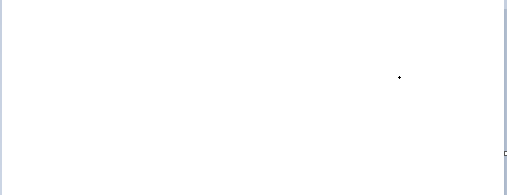
\includegraphics[width=\columnwidth]{figs/box.png}
	\caption{Spatial attention pooling to balance edge alignment and stroke ambiguity at different facial regions. }
	\label{fig:sap}
\end{figure}



%%% \subsubsection{Spatial Local Respond Normalization}
%\input{slrn}
%%% \subsubsection{Losses}
% !TeX root = SketchFace.tex

\subsubsection{Losses}
\td{generator feature matching effect and losses summary}



Let $G_q(·)$ be the  feature maps of the $q$th generator layer.
Given an input sketch $s$ and the corresponding deformed sketch $s'$, we compute the generator feature matching loss as:

\begin{equation}
	\label{eqn:loss_GFM}
	\mathcal{L}_{GFM}(G)=\mathbb{E}_{\mathbf{s}\sim p_{data}(s)} \frac{1}{N_Q} \sum_{q\in Q}  \frac{1}{N_Q} \|G_q(s)-G_q(s') \|_1,
\end{equation}

where $n_q$ denotes the number of elements of $G_q$, $Q$ indicates a set of the selected generator layers for computing this loss and the size of $Q$ is $N_Q$. 
We select \td{the xxx layers} of the generator in our experiments.

Besides the generator feature matching loss $\mathcal{L}_{GFM}(G)$, for generator $G$ and multi-scale discriminator $D={D_k | k=1,2,...,N_D}$, the adversarial loss $\mathcal{L}_{GAN}(G, D)$ and the discriminator feature matching loss $\mathcal{L}_{DFM}(G, D)$ are computed as the same form as those in pix2pixHD~\cite{pix2pixHD}.
%
The objective of the proposed model is:

\begin{equation}
	\label{eqn:new_minmax_game}
	\min_G \max_{D} \mathcal{L}_{GAN}(G, D)+\lambda \mathcal{L}_{DFM}(G, D) +\mu \mathcal{L}_{GFM}(G).
\end{equation}

where $\lambda$ and $\mu$ are the weights for balancing different losses. We set $\lambda=\td{xxx}$ and $\mu=\td{xxx}$ in our experiments.




%\paragraph{Sketch Data Generation}
%Four options to generate sketches: Canny, HED, AutoTrace [Web..], and Contour. 

. 